\documentclass[a4paper]{article}


\usepackage{arxiv}

\usepackage[utf8]{inputenc} % allow utf-8 input
\usepackage[T1]{fontenc}    % use 8-bit T1 fonts
\usepackage[colorlinks = true,
            linkcolor = blue,
            urlcolor  = blue,
            citecolor = blue,
            anchorcolor = blue]{hyperref}       % hyperlinks
\usepackage{url}            % simple URL typesetting
\usepackage{booktabs}       % professional-quality tables
\usepackage{amsfonts}       % blackboard math symbols
\usepackage{nicefrac}       % compact symbols for 1/2, etc.
\usepackage{microtype}      % microtypography
\usepackage{lipsum}
\usepackage{amsmath}
\usepackage{graphicx}
\usepackage{subcaption}
\usepackage{floatrow}
\usepackage{float}


\DeclareMathOperator*{\argmax}{arg\,max}
\DeclareMathOperator*{\argmin}{arg\,min}


% Default fixed font does not support bold face
\DeclareFixedFont{\ttb}{T1}{txtt}{bx}{n}{12} % for bold
\DeclareFixedFont{\ttm}{T1}{txtt}{m}{n}{12}  % for normal

% Custom colors
\usepackage{color}
\definecolor{deepblue}{rgb}{0,0,0.5}
\definecolor{deepred}{rgb}{0.6,0,0}
\definecolor{deepgreen}{rgb}{0,0.5,0}

\usepackage{listings}

% Python style for highlighting
\newcommand\pythonstyle{\lstset{
language=Python,
basicstyle=\ttm,
otherkeywords={self},             % Add keywords here
keywordstyle=\ttb\color{deepblue},
emph={MyClass,__init__},          % Custom highlighting
emphstyle=\ttb\color{deepred},    % Custom highlighting style
stringstyle=\color{deepgreen},
frame=tb,                         % Any extra options here
showstringspaces=false            % 
}}


% Python environment
\lstnewenvironment{python}[1][]
{
\pythonstyle
\lstset{#1}
}
{}

% Python for external files
\newcommand\pythonexternal[2][]{{
\pythonstyle
\lstinputlisting[#1]{#2}}}

% Python for inline
\newcommand\pythoninline[1]{{\pythonstyle\lstinline!#1!}}



\title{Generisanje slika korišćenjem GAN}


\author{
  Jovan Ležaja \\
  brindeksa\\
  Matematički fakultet, Beograd \\
  \texttt{navoj96@gmail.com} \\
  %% examples of more authors
   \And
 Aleksandar Vračarević \\
  434/2016\\
  Matematički fakultet, Beograd \\
  \texttt{vracarevicaleksandar@gmail.com} 
}

\begin{document}
\maketitle

\begin{abstract}
\lipsum[1]
\end{abstract}
\setcounter{tocdepth}{2}
\renewcommand{\contentsname}{Sadržaj}
\tableofcontents

\newpage

% keywords can be removed
%\keywords{GAN \and Generative models \and Soft computing \and Artificial Neural Networks \and Convolutional Neural Networks}


\section{Uvod}
\lipsum[2]



\section{Generativni modeli}
\label{sec:genmodeli}

Problem koji generativni modeli pokušavaju da reše odnosi se na učenje nekog skupa osobina na osnovu ulaznih podataka i korišćenje tih osobina za modelovanje novih podataka nalik na onima koji su zatečeni u originalnom skupu. Ovaj problem može se predstaviti uz pomoć verovatnoće. Ukoliko trening podaci pripadaju nekoj raspodeli $p_{stvarno}(x)$ a generisani podaci pripadaju raspodeli $p_{generisano}(x)$, cilj je da veštačka raspodela $p_{generisano}(x)$ bude što sličnija raspodeli $p_{stvarno}(x)$. Dakle, generativni model se "trudi" da na osnovu podataka za trening generiše nove uzorke koji pripadaju istoj raspodeli. Primetimo da u nekim slučajevima nije neophodno eksplicitno pronaći raspodelu modela. Naime, nekada je dovoljno da model ima sposobnost da izvlači uzorke koji pripadaju raspodeli $p_{generisano}(x)$ bez toga da se ista eksplicitno definiše. Naše rešenje je zasnovano na ovom pristupu. 
%           Poređenje?
\subsection{Podela generativnih modela}
\label{subsec:podela}

Da bi se olakšalo poređenje različitih modela, potrebno ih je generalizovati na one koji koriste \textbf{metodu maksimalne verodostojnosti}\footnote{Mnogi modeli ne koriste ovu metodu, ali se mogu preraditi tako da je koriste, što je slučaj i sa GAN\cite{nipstut}.} i ignorisati one koji imaju drugačiji pristup. Osnovna ideja ove metode je da se procenjuje parametar $\theta$ za koji \textbf{funkcija verodostojnosti} dostiže maksimalnu vrednost, odnosno traži se vrednost parametra za koju je najverovatnije da će se ostvariti realizovani uzorak. Funkcija verodostojnosti definiše se kao $\prod_{i=1}^{m}p_{model}(x_i ; \theta)$. Dakle, ocenjujemo parametar $\hat{\theta}$: 
\begin{align*}
\label{eq:loglikelihood}
    \hat{\theta} =  \argmax_{\theta}\prod_{i=1}^{m}p_{model}(x_i ; \theta) =\\ \argmax_{\theta}\log\prod_{i=1}^{m}p_{model}(x_i ; \theta) =\\ \argmax_{\theta}\sum_{i=1}^{m}\log{p_{model}(x_i ; \theta)}
\end{align*}

%TODO: preformulisati ovo oko trening skupa, nisam bas siguran da je tacno
Uvođenje logaritama olakšava račun jer se umesto proizvoda izračunava suma koja je otpornija na prisustvo veoma malih vrednosti. 
Drugi način formulacije problema je preko minimizovanja \textbf{Kulbak-Lajblerove divergencije} (eng.~{\em Kullback-Leibler divergence}) između raspodele podataka iz trening skupa i raspodele koju generiše model: 
$$ \hat{\theta} = \argmin_{\theta}D_{KL}(p_{podaci}(x)||p_{model}(x;\theta)) $$ gde je $$D_{KL}(p_{podaci}(x)||p_{model}(x;\theta)) = \sum_{i=q}^{N}p_{podaci}(x_i)log\frac{p_{podaci}(x)}{p_{model}(x;\theta)} = E[\log{p_{podaci}(x)} - \log{p_{model}(x;\theta)}]$$
U praksi se ne zna raspodela $p_{podaci}$ direktno, već su dostupni uzorci iz te raspodele. Na osnovu tih uzoraka, pravi se empirijska raspodela $\hat{p}_{podaci}$ koja aproksimira $p_{podaci}$. Minimizacija Kulbak-Lajblerove divergencije ekvivalentna između $\hat{p}_{podaci}$ i $p_{model}$  je maksimizovanju logaritma verodostojnosti trening skupa. \\ %\ref{eq:loglikelihood}h %gornja jednacina?

Na slici \ref{fig:taxonomy} je prikazana podela generativnih modela zasnovanih na metodi maksimalne verodostojnosti koju predlaže Ijan Gudfelou (eng.~{\em Ian Goodfellow}) u \cite{nipstut}, ali će u nastavku rada fokus biti stavljen na GAN (eng.~{\em Generative Adversarial Networks}).  

%varijacione autoenkodere (eng.~{\em Variational Autoencoders}) i 

\begin{figure}
  \centering
  \includegraphics[width=0.5\textwidth]{taxonomy.png}
  \caption{Podela generativnih modela.}
  \label{fig:taxonomy}
\end{figure}
    
%\subsubsection{Varijacioni autoenkoderi}

%Varijacioni autoenkoderi spadaju u grupu modela koji eksplicitno definišu funkciju raspodele $p_{model}(x;\theta)$, s time da se ta raspodela aproksimira kako bi se verodostojnost maksimizovala.  

\subsection{GAN}
Ideja iza GAN modela je zapravo igra između dva igrača, od kojih je jedan \textbf{generator}, a drugi \textbf{diskriminator}. Generator pokušava da sintetiše podatke koji prate raspodelu trening podataka, odnosno trudi se da na što bolji način reprodukuje originalne podatke. Diskriminator je binarni klasifikator koji pokušava da razluči da li su podaci lažne ili prave. Generatoru je cilj da generiše dovoljno dobre podatke koje diskriminator neće uspeti da klasifikuje sa velikom sigurnošću. U primeru koji je naveden u \cite{goodfellow2014generative} se generator predstavlja kao tim falsifikatora koji se trude da naprave lažan novac, dok je diskriminator policija i pokušava da razotkrije falsifikovan novac, a dopusti pravi. Ovo nadmetanje forsira oba igrača da se unapređuju sve dok generisane novčanice ne mogu da se razlikuju od pravih.   

I generator i diskriminator su višeslojni perceptroni predstavljeni funkcijama $G(z,\theta_{g})$ i $D(x, \theta_{x})$ redom. Izlaz funkcije diskriminatora je verovatnoća da je $x$ pravi podatak, a ne lažni, generisani. 
Ukoliko matematički formulišemo ovu igru, videćemo sličnost sa jednačinom INSERT:REF:
$$\argmin_{G}\argmax_{D}V(D,G) = E_{x \sim\ p_{podaci}(x)}[\log{D(x)}] + E_{z \sim\ p_{generator}(z)}[\log{1-D(G(z))}]$$

U praksi se javlja problem sa ovom jednačinom prilikom treniranja. Naime, u početku je G loš, a D može s velikom sigurnošću da odbaci podatke koje generiše G jer su očigledno različiti od pravih. U tom scenariju, $\log{1-D(G(z))}$ je blisko nuli pa G nema dobre izglede za poboljšanje. Kako bi se ovaj problem rešio, G se ne trenira da minimizuje $\log{1-D(G(z))}$, već da maksimizuje $\log{D(G(z))}$. Ovaj pristup se ponaša isto kao i originalan, ali su gradijenti za G u početku mnogo pogodniji za trening.

\section{Implementacija}
Koristeći se programskim jezikom Python, bibliotekom pytorch i idejama ..., pokušaćemo da, na više različitih načina, konstruišemo generativni model. Prvi od njih se najvećim delom zasniva na \cite{goodfellow2014generative} i predstavlja najosnovniju, "vanila" verziju modela. Nakon toga, prateći savete iz ... , pokušavamo da poboljšamo model. Na samom kraju biće prikazani i neki napredniji koncepti u rešavanju problema generisanja podataka korišćenjem GAN-a. U okviru svakog pristupa, biće prikazane korišćene transformacije podataka koje mogu imati znatan uticaj na kvalitet modela. %i fotografije automobila čije dimenzije pripadaju skupu [min_w,max_w] X [min_h,max_h] %Pomenute slike ćemo obraditi na nekoliko načina kako bismo poboljšali kvalitet dobijenog generatora. 

\subsection{Vanila GAN}
 Skup podataka koji pokušavamo da reprodukujemo sastoji se od skoro 16.000 slika mačijih lica u formatu 64x64. Iako su originalne slike u boji, mi smo primenili transformaciju Grayscale kako bismo smanjili vreme treninga modela\footnote{Naime, umesto da koristimo tri kanala i 64x64x3 piksela, koristimo samo 64x64x1 piksela i time smanjujemo potrebno vreme racunanja.}. Nakon toga, podaci su normalizovani tako da imaju srednju vrednost 0.5 i disperziju 0.5 opet u svrhu lakše i bolje obrade. Generator je potpuno povezana mreža koja prima vektor od 100 nasumičnih brojeva i propušta ih kroz 4 skrivena sloja. Izlaz iz generatora je 4096 piksela koji predstavljaju generisanu sliku. Diskriminator je takođe potpuno povezana mreža koja prihvata 4096 piksela, odnosno generisanu ili pravu sliku i nakon prolaska kroz 4 skrivena sloja kao odgovor daje svoju procenu da li je ulazna slika prava ili generisana. U skrivenim slojevima obe mreže korišćena je LeakyReLU funkcija aktivacije. U završnom sloju generatora koristi se hiperbolični tangens, a diskriminator u svom poslednjem sloju ima sigmoidnu funkciju aktivacije.\footnote{U originalnom radu, generator koristi mešavinu ReLU i sigmoidnih aktivacionih funkcija, a diskriminator koristi maxout funkciju aktivacije.} Procenat čvorova mreže koji se odbacuju, odnosno dropaut (eng.~{\em dropout}) je 0.3. Trening se zasniva na algoritmu INSERT:REF. Zbog vremenskih i hardverskih ograničenja, treniranje je dva puta izvršeno u 30 epoha. Za vizualizaciju funkcija gubitka korišćena je biblioteka tensorboardX.
 
 \begin{figure}[h!]
     \centering
     \begin{subfigure}{0.4\linewidth}
     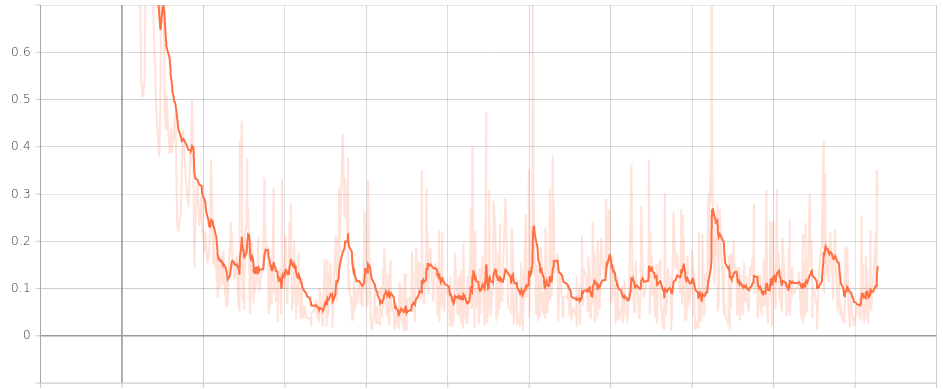
\includegraphics[width=\linewidth]{D_error_1.png}
     \caption{Greška diskriminatora u prvom prolazu}
     \end{subfigure}
     \begin{subfigure}{0.4\linewidth}
     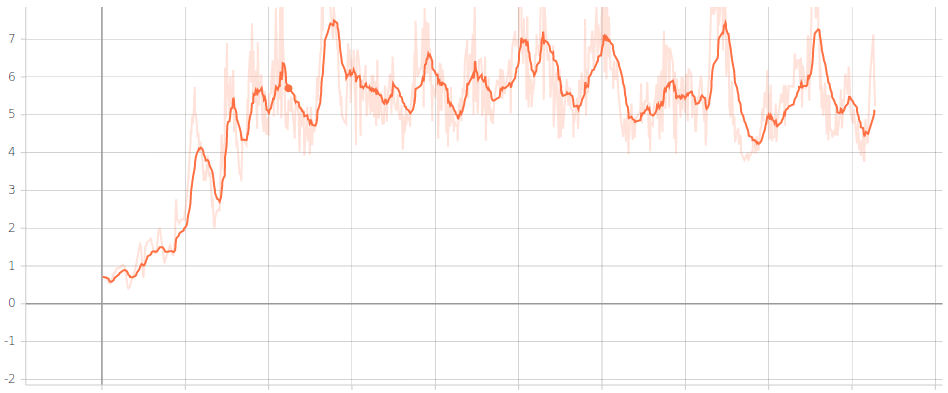
\includegraphics[width=\linewidth]{G_error_1.png}
     \caption{Greška generatora u prvom prolazu}
     \end{subfigure}
 \end{figure}
 
  \begin{figure}[h!]
     \centering
     \begin{subfigure}{0.4\linewidth}
     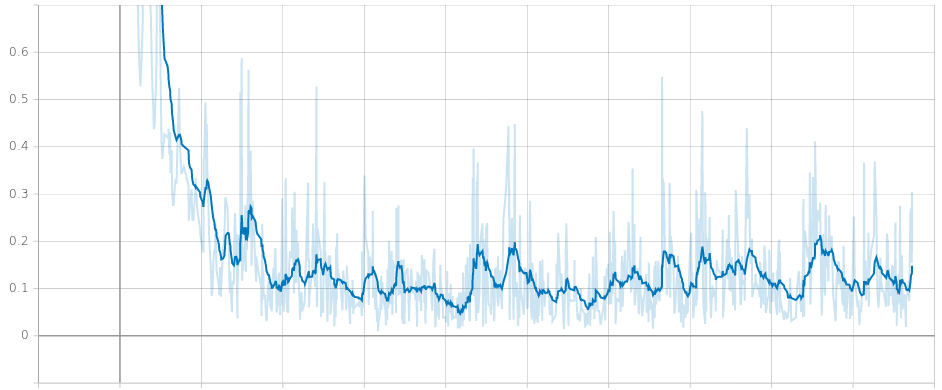
\includegraphics[width=\linewidth]{D_error_2.png}
     \caption{Greška diskriminatora u drugom prolazu}
     \end{subfigure}
     \begin{subfigure}{0.4\linewidth}
     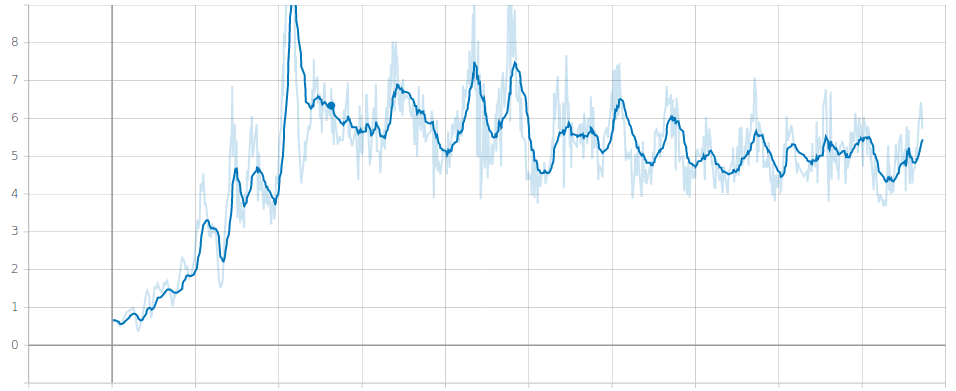
\includegraphics[width=\linewidth]{G_error_2.png}
     \caption{Greška generatora u drugom prolazu}
     \end{subfigure}
 \end{figure}

Sa grafika grešaka generatora i diskriminatora vidimo da je u početku treninga diskriminator dosta loš i ne uspeva da raspozna stvarne od lažnih slika, dok generator ima veoma nisku vrednost greške. Kako vreme prolazi, vidimo da se diskriminator drastično poboljšava i greška mu se snižava, dok greška generatora raste. Kako bi generisane slike bile optimalne, potrebno je da dođe do konvergencije između grešaka generatora i diskriminatora, što se u našem slučaju nije dogodilo. Naime, vidimo da se diskriminator veoma brzo poboljša što dovodi do povećanja greške generatora, ali se na kraju ove dve veličine ne izjednače kao što bi se u optimalnom slučaju dogodilo. Ostaje pitanje da li bi treniranje u više epoha dovelo do boljih rezultata ili je loš odabir parametara algoritma učenja doveo do ovakvih rezultata. Napomenimo da je nad prikazanim graficima primenjena \href{https://github.com/tensorflow/tensorboard/blob/f801ebf1f9fbfe2baee1ddd65714d0bccc640fb1/tensorboard/plugins/scalar/vz_line_chart/vz-line-chart.ts#L42}{funkcija glačanja} (eng.~{\em smoothing}) sa parametrom 0.9 kako bi se lakše uočio trend kretanja grešaka jer je puno šuma prisutno na originalnom grafiku (linija slabijeg intenziteta predstavlja grafik pre glačanja).  

Uprkos tome što greške nisu konvergirale, rezultujuće slike blago podsećaju na lica mačaka. Kao što smo već spomenuli, smatramo da bi veći broj epoha za treniranje doveo do boljih rezultata. Ispod su predstavljene mačke generisane od strane naše implementacije GAN-a. 

\begin{figure}[h!]
    \centering
    \begin{subfigure}{0.3\linewidth}
     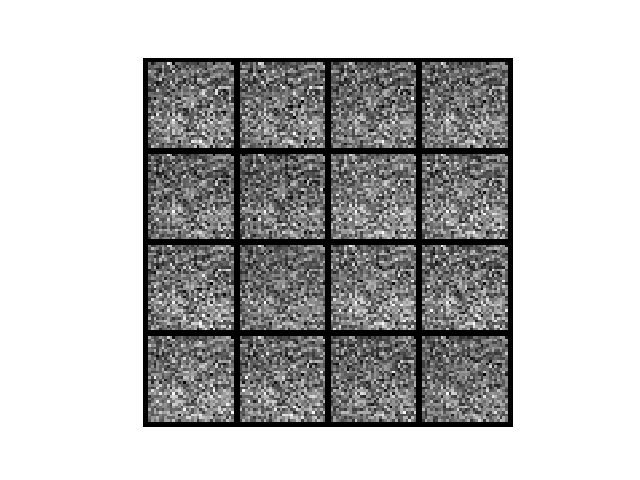
\includegraphics[width=\linewidth]{_epoch_0_batch_100.png}
     \caption{Generisane slike u 1. epohi}
     \end{subfigure}
     \begin{subfigure}{0.3\linewidth}
     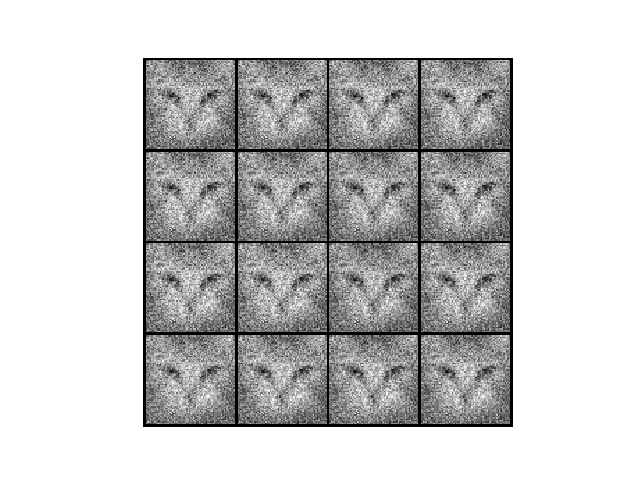
\includegraphics[width=\linewidth]{_epoch_15_batch_150.png}
     \caption{Generisane slike u 15. epohi}
     \end{subfigure}
     \begin{subfigure}{0.3\linewidth}
     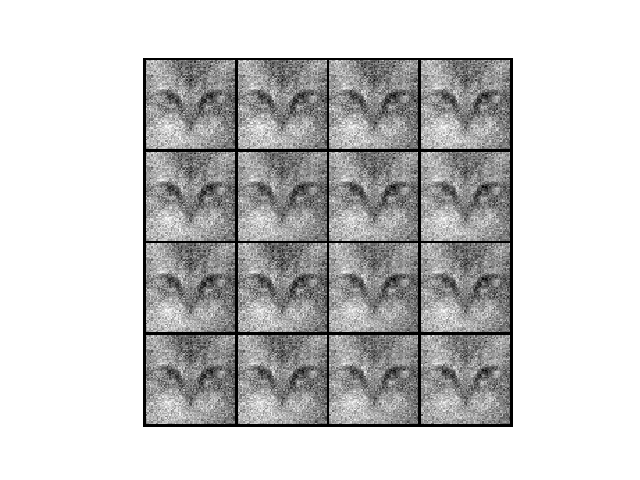
\includegraphics[width=\linewidth]{_epoch_28_batch_150.png}
     \caption{Generisane slike u 28. epohi}
     \end{subfigure}
    \label{fig:cats_first_run}
    \caption{Prvi prolaz}
\end{figure}

\begin{figure}[h!]
    \centering
    \begin{subfigure}{0.3\linewidth}
     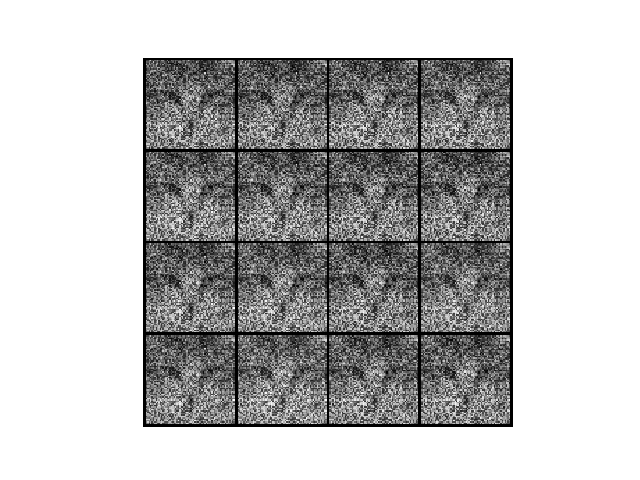
\includegraphics[width=\linewidth]{__epoch_0_batch_100.png}
     \caption{Generisane slike u 1. epohi}
     \end{subfigure}
     \begin{subfigure}{0.3\linewidth}
     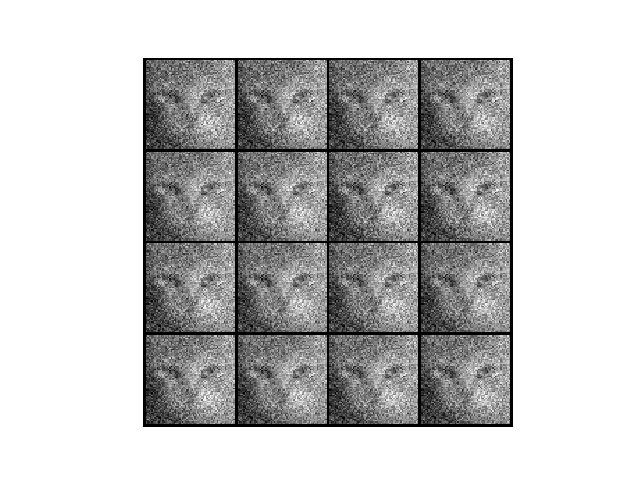
\includegraphics[width=\linewidth]{__epoch_15_batch_150.png}
     \caption{Generisane slike u 15. epohi}
     \end{subfigure}
     \begin{subfigure}{0.3\linewidth}
     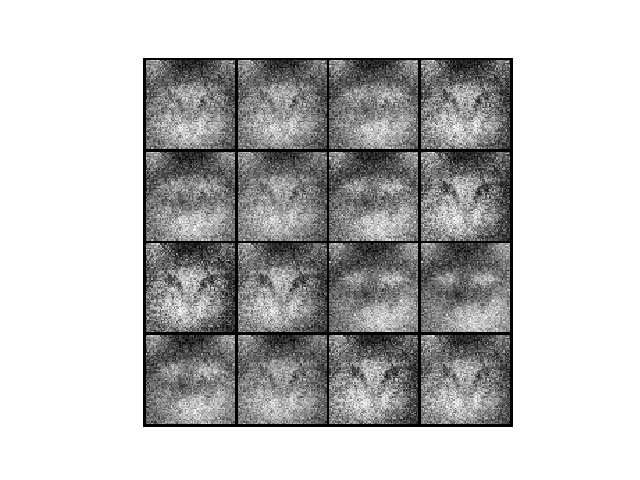
\includegraphics[width=\linewidth]{__epoch_30_batch_100.png}
     \caption{Generisane slike u 30. epohi}
     \end{subfigure}
    \label{fig:cats_second_run}
    \caption{Drugi prolaz}
\end{figure}

Zaključujemo da je, zarad poboljšanja rezultata, neophodo istražiti drugačije arhitekture, dodatno pripremiti podatke pre početka treninga i trenirati veći broj epoha što će u ostatku rada i biti učinjeno.

\subsection{Poboljšanja}


\bibliographystyle{unsrt}  
\renewcommand{\refname}{Literatura}
\newpage
\bibliography{literatura}
\end{document}